\begin{savequote}[75mm]

... As for me, nothing in the universe can be the same if somewhere, no one knows where, a sheep we never saw has or has not eaten a rose....
Look up at the sky. Ask yourself, ``Has the sheep eaten the flower or not?" And you'll see how everything changes....
And no grown-up will ever understand how such a thing could be so important!
\qauthor{Antoine de Saint-Exup{\^e}ry (The Little Prince)}
\end{savequote}


\chapter{Introduction}
\label{introduction}

\section{A Brief History of Galaxy Evolution}

\subsection{The Discovery of Galaxies}
One of the momentous shifts in scientific thinking was the realization that our Sun might be one of many stars in the Universe. From this sprung the idea that perhaps the gravitationally bound system of stars, stellar remnants, gas and dust that the Sun is a part of is one of many such structures known as galaxies. The bright band of stars and dust that we observe in the night sky, which we now know as our own galaxy, the Milky Way, has been a puzzling topic since ancient times. The Greek philosopher Democritus is known to have speculated that this might be a band of distant stars but the thought was left by the wayside with the advent of Aristotelian physics. The astronomers of medieval Islam, such as Alhazen, al-Biruni and Ibn-Bajjah, centuries later, also hypothesized that the Milky Way was made of many stars such as our own Sun. However, observational proof for this came only in the 17th century when the Italian astronomer, Galileo Galelei pointed his telescope at this band and confirmed that the Milky Way was indeed made up of a huge number of faint stars.\\

Since the debate on a geocentric versus heliocentric Universe was still ongoing, Galileo's observations weren't given credence until more than century later, during which time, the development of Keplerian orbital mechanics and Newtonian Theory of Gravitation had resulted in a successful explanation of the Solar System and its dynamics. The idea that the galaxy might be a rotating configuration of a huge number of stars held together by gravitational forces that contained smaller gravitationally bound configurations such as our Solar System was first theorized by the English astronomer, Thomas Wright, in 1750. On the heels of his observation that the faint (then so-called) ``nebulae" observed might be distant galaxies that came out of ``external creations", philosopher Immannuel Kant hypothesized the existence of many such ``island Universes" and speculated that these could potentially form and evolve independently from our own, thus laying the underpinnings of the study of galaxy formation and evolution.\\

\subsection{Early Studies of Galaxies}

William Herschel, in the 1780s, surveyed the stars in the Milky Way in multiple directions and discovered that the density of stars was greater on one side than the other. One of the earliest catalogues of galaxy-like objects was developed by Charles Messier, also towards the end of the 18th century, following which William Herschel assembled a catalog of 5000 nebulae. In the 19th century, with advances in optics and instrumentation, the first telescope to distinguish between elliptical and spiral galaxies was built by Lord Rosse. Additionally, this telescope could resolve point sources within the nebulae, thus confirming that galaxies were indeed ``island universes" as Wright and Kant had surmised.\\

In early 20th century, astronomers were beginning to get interested in the chemical composition of these nebulae and started recording their spectra. With the advent of Einstein's Special Theory of Relativity, one could calculate the radial velocity of a ``nebula" based on how its spectrum is Doppler-shifted. And so it happened that the American astronomer, Vesto Slipher, became the first person to measure galactic redshifts in 1912. While studying the chemical composition of bright spiral nebulae, he noticed that they were all highly Doppler-shifted, with estimated radial velocities that were much higher than the velocities of stars in the Milky Way. He also noticed that there were more ``red-shifted" (i.e. moving away from us) nebulae than ``blue-shifted" ones, an observation that would later propel Edwin Hubble to propose that the Universe was expanding.\\

In the 1920s, a series of observations made by Edwin Hubble, Ernst Opik, etc., confirmed that Andromeda was not a part of the Milky Way and was a galaxy is its own right, thus effectively settling the ``Great Debate" of the times and confirming that our galaxy was just one of many galaxies in the Universe. Georges Lema{\'i}tre, a Belgian physicist, predicted, on theoretical grounds rooted in Einstein's General Theory of Relativity, that the redshifts of galaxies should increase with distance. In 1929, Edwin Hubble looked at the distances and velocities of 46 galaxies and observed the same \citep{1929PNAS...15..168H}: that their radial velocities increased with distance from us, thus theorizing what we know today as Hubble's Law (or alternately, the Hubble-Lema{\'i}tre Law). Edwin Hubble further analyzed the morphologies of these galaxies and came up with the Hubble Sequence, a classification of galaxy morphology (Fig. \ref{fig:hubble_classification}). The Swiss astrophysicist, Fritz Zwicky, in 1933, while studying galaxy clusters, noticed that the orbits of the galaxies were not accounted for by the mass of its luminous components, leading him to believe that there must be some ``missing" mass \citep{1937ApJ....86..217Z} that does not interact electromagnetically, thus remaining unseen and termed it \emph{dunkle Materie}, i.e.,'`dark matter".\\

Thus with the emergence of new theories of spacetime, an expanding Universe that (as it was termed later) began with a ``big bang", the existence of matter that doesn't interact electromagnetically, the study of galaxies in the 1930s set in motion a paradigm shift for astronomy and cosmology. The new questions were: How were the earliest galaxies formed? What would explain the diversity in morphologies seen in galaxies today? Is the Universe set to expand indefinitely? What drives the expansion of the Universe? What is dark matter? If the Universe's origins were homogeneous, how do we explain the heterogenous nature of the populations of galaxies seen?\\

\subsection{Galaxy Evolution and Cosmology}

The explorations in the latter half of the 20th century confirmed a few of the hypotheses discussed above, along with answering a few of those questions. In the 1960s and 1970s, Vera Rubin, Kent Ford, and Ken Freeman analyzed rotation curves of spiral galaxies and provided strong evidence for the existence of dark matter \citep{freeman_disks_1970-1}. Rubin inferred that most galaxies contain around six times as much dark matter as visible mass \citep{rubin_rotational_1980}, thus placing new constraints on galaxy formation and evolution in the Universe.\\

The two predominant theories of the origin of the Universe were: the ``Big Bang Theory", originally proposed by Georges Lema{\'i}tre, and the ``Steady State Theory" (essentially an unchanging Universe whose density remains the same in spite of expansion due to continuous creation of matter) proposed by Fred Hoyle. However, with theories of Big Bang Nucleosynthesis (the $\alpha\beta\gamma$ paper; \citealt{alpher_origin_1948}) that successfully explained how the elements of the of the Universe came to be formed after the Big Bang and radio source counts which were also correctly accounted for by the Big Bang Theory swung cosmologists to favor this over the Steady State Theory. The final nail in the coffin was the successful detection of the Cosmic Microwave Background (CMB), predicted by the Big Bang Theory \citep{1965ApJ...142..419P}. According to the Big Bang Theory, the early Universe cools from a very hot state and remains an ionized plasma for the first few hundred thousand years (until redshift $z\sim 1100$). The emission from this era should be a Planck spectrum of the plasma at about the time that hydrogen recombines, redshifted due to the universe's expansion since then. This model predicts a spectrum peaking at near microwave wavelengths today, and the CMB is indeed detectable as a very low energy radiation with a blackbody temperature of \~ 3K.\\

The discovery of dark matter coupled with the confirmation of the Big Bang Theory necessitated a theory of dark matter that would successfully explain the observable Universe. In the 1980s, competing theories of hot and cold dark matter \citep{1985ApJ...292..371D} were proposed. Eventually the cold dark matter theories won out as their prediction of the anisotropies in the CMB \citep{peebles_large-scale_1982} were successfully verified by the Cosmic Background Explorer (COBE) probe \citep{smoot92a} in combination with other data sets.\\

Before the turn of the century, the remarkable discovery of the accelerating universe \citep{Riess:1998cb} resulted in the resurrection of Einstein's cosmological constant and effectively confirmed $\Lambda$CDM as the clear winner among the cold dark matter models. The Big Bang Theory, together with the $\Lambda$CDM model, forms much of the basis of modern cosmology and the foundations for theories of galaxy formation and evolution.\\

\section{Galaxy Formation and Evolution}

\subsection{Structure Formation in the Universe}
The current model of cosmology suggests that there was a single event, the so-called ``Big Bang" which resulted in the appearance of expanding space-time containing radiation, followed by an exponential expansion of space known as cosmic inflation \citep{PhysRevD.23.347} which established the initial properties of the Universe as being homogeneous, isotropic and flat. Tiny perturbations in this early Universe are responsible for structure formation. Cosmic inflation also explains the fact that these tiny quantum fluctuations grow into slight ripples of over-density and under-density thus seeding the early stages of structure formation in the Universe.\\

From a predominantly radiation-dominated Universe, with expansion, the density of radiation drops steeply leading to a the matter-radiation equality at ~ 50,000 years after the Big Bang. Since dark matter only interacts gravitationally, the dark matter ripples from the fluctuations form compact structures more freely as they are not opposed by other forces such as radiation pressure.\\

About 380,000 years after the Big Bang, the expansion of the Universe resulted in a lowering of density as well as a cooling down of its temperature to a point where protons and electrons in this plasma soup start combining to form the neutral hydrogen. Electrons decouple from the photons (these decoupled photons are what we detect as the CMB today) and the baryonic matter is now free to collapse under gravity creating local over-densities.\\

As fluctuations continue to grow, ever larger scales enter the non-linear regime of structure formation where dense concentrations of matter (dark and baryonic alike) get progressively denser. 
Dark matter begins to collapse into structures known as halos, and baryons fall with the dark matter into these halos. These structures arrange themselves into gravitationally stable configurations, a process known as virialization.
The result of this process gives rise to a Universe that resembles a web (the cosmic web) with sheets and filaments of dark matter, creating a skeletal backbone in which star formation and galaxy formation eventually occur.

Within the dark matter halos baryonic matter can, when it becomes dense enough, additionally lose energy by radiation and can sink further into regions of high over-density. 
The stars and galaxies have their origins in these structures and are the resulting of the cooling of baryons deep in the potential wells of dark matter halos.

While a short summary of how galaxies form would be that the collapse of baryonic matter within dark matter halos results in disk-like structures that then collapse on small scales to form stars, the mechanisms by which this happens is still a topic of debate among astrophysicists. While a top-down scenario, wherein disk galaxies were formed from the collapse of a single large cloud of gas \citep{1962ApJ...136..748E}, captures some stages of galaxy formation well, in fact both theory and observations suggest that galaxies grow hierarchically --- small galaxies form and merge into larger ones --- which complexifies the picture. Meanwhile, the overall efficiency with which baryons form stars depends strongly on the halo mass (e.g. \citealt{behroozi_comprehensive_2010}), peaking at masses similar to that of the Milky Way. As \citet{somerville15a} describe, this dependence probably arises from processes that suppress star formation at lower masses (perhaps due to supernova feedback) and at higher masses (perhaps due to feedback from accreting supermassive black holes).

% Prior to the establishment of $\Lambda$CDM as the dominant cosmological model, the popular theory of galaxy formation was the top-down scenario \citep{1978ApJ...225..357S} which proposed that disk galaxies were formed from the collapse of a single large cloud of gas \citep{1962ApJ...136..748E} into disks that pushed the dark matter out into halos. The cooling of this rotating disk results in gravitational instabilities that causes smaller clumps of clouds to collapse to form stars. However, the natural prediction of $\Lambda$CDM is a bottom-up scenario wherein the dark matter halos form and 
% (\citet{0004-637X-490-2-493, 2015PNAS..11212249W}) before the formation of the galactic disks.\\

Since we are limited in our observations by the fact that we cannot observe galaxies in a time-resolved fashion (the time scales are too long), theories regarding galaxy formation rely computational simulations that evolve the initial conditions to the present day. We can compare the galaxies at each epoch to the populations observed at different redshift, assuming large scale homogeneity. As \citet{somerville15a} describe, these simulations incorporate the physics of $\Lambda$CDM, magnetohydrodynamics, and gravitation. Additionally, these models need to account for a variety of processes on subresolution scales that involve star formation, stellar and AGN feedback, and gas cooling to be able to correctly predict the observed Universe.\\

\begin{figure}
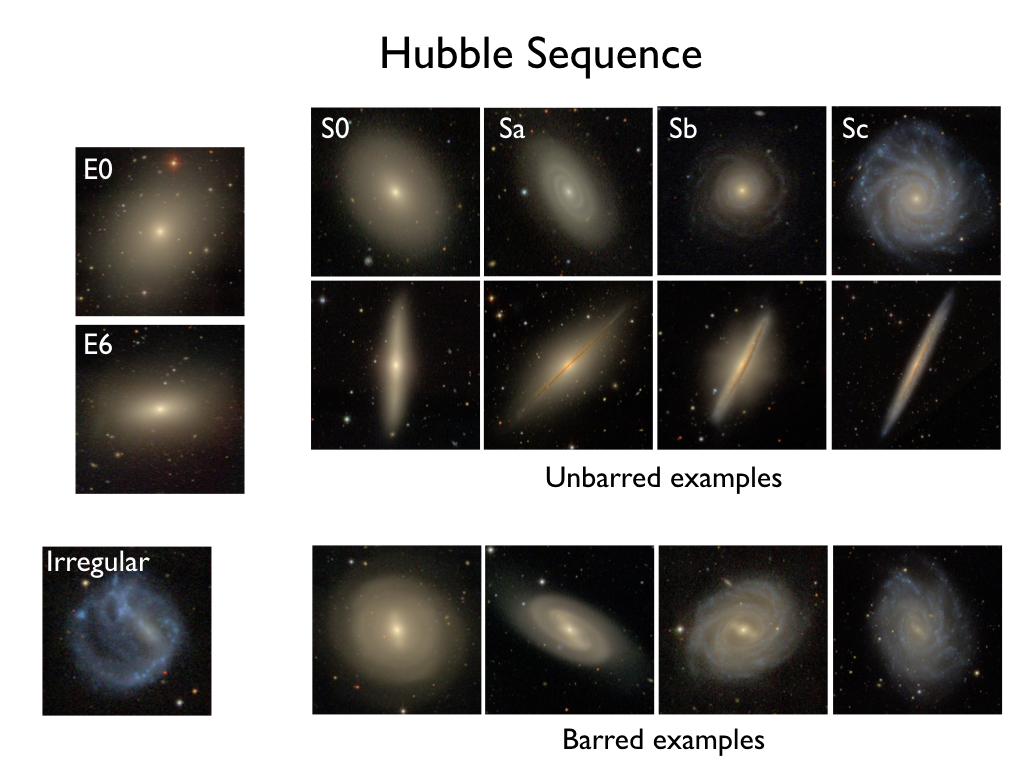
\includegraphics[width=\textwidth]{figures/hubble.jpeg}
\caption[ The Hubble Sequence: A classification scheme for galaxy morphologies (Photo credit: ?)]
{The Hubble Sequence: A classification scheme for galaxy morphologies (Photo credit: ?)
\label{fig:hubble_classification}}
\end{figure}

Thus, there are still many questions to be answered including and not limited to: how and where the baryons collapse, how galactic disks stabilize, the drivers and mechanisms of galactic feedback and what ultimately causes the relative frequency of different galaxy types in the observable Universe. There are thus many holes in this narrative of galaxy formation and evolution and astronomers are working to bridge this gap in two main ways: from the observational side, this involves accurate measurements of galaxy properties across cosmic time and from the (theoretical) side of computational astrophysics, this involves fine-tuning the sub-grid models of galaxy formation and evolution simulations so as to be able to reproduce the estimated from the properties. These both take from and in turn inform the parameters in the $\Lambda$CDM model of the Universe that cosmologists are engaged in refining.\\

\subsection{Galaxies in the Observable Universe}

The classification of galaxies based on their most obvious attribute, the morphologies of their luminous components, was invented by Edwin Hubble in 1926. The classification scheme is based on the relative sizes and of the bulges and disks in galaxies and broadly encompasses four types of morphologies: elliptical, lenticular, spiral and irregular (Fig. \ref{fig:hubble_classification}). Galaxy morphologies are strongly correlated with their other physical properties such as luminosity, age, chemical composition, star formation histories and kinematics (\citealt{roberts94a}). The bulges usually contain older, redder stars and the disks are characterized by mixed stellar populations along with gas and dust. The disks may also contain spiral arms which usually contain pockets of star formation activity as is evident by their blueness. Elliptical galaxies have almost no disk, lenticulars are ellipticals with thin disks (lentil-shaped!) and spirals have a bulge and disk with spiral arms. Irregulars are akin to spirals but as their name suggests, have ill-defined bulges, disks and spiral arms. Early ideas about galaxy evolution suggested that galaxies formed as ellipticals or lenticulars (referred to as `early-type' galaxies) and later evolved into spirals or irregulars (referred to as `late-type' galaxies) and while there are strong correlations between galactic structure and their star formation rates, it is now known that this is in general untrue.\\

\begin{figure}
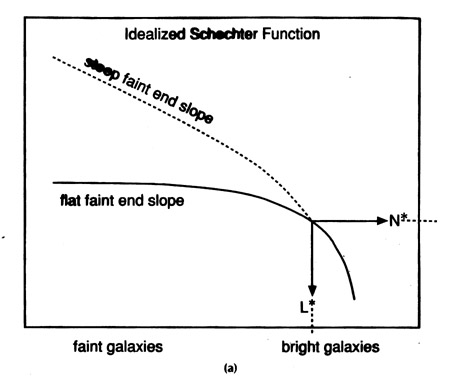
\includegraphics[width=\textwidth]{figures/luminosity_function}
\caption[PLACEHOLDER FIGURE TBD: Schematic illustration the distribution of luminosities of galaxies in the observed Universe]
{ PLACEHOLDER FIGURE TBD: Schematic illustration the distribution of luminosities of galaxies in the observed Universe
\label{fig:lum_func}}
\end{figure}


The total amount of light we observe emanating from a galaxy is the second obvious trait that lends itself to comparison. This can be quantified as ``Luminosity", the amount of energy emitted by a star in unit time, measure in units of $L_{\odot}$ and serves as a reasonable proxy for either stellar mass or the current star formation activity or both. Observations reveal that fainter galaxies and more frequent than spiral galaxies as bright as our own. Very bright big ellipticals are much rarer than both. While the distribution of luminosities of galaxies in the observable Universe is pretty informative, when coupled with the relative abundances of galaxies in volume, we get a more informative constraint on evolution of the galaxy, namely, the Luminosity Function. The relative volume densities of galaxies, according to the physics of how galaxies virialize (i.e. stabilize and internally decouple from cosmic expansion), at any given time, is constrained by the mass of the galaxy. The relative volume density of galaxies within a given luminosity bin as a function of luminosity is known as the Luminosity Function (\citet{1988MNRAS.232..431E, 2003ApJ...599...38B}), which informs not only galaxy evolution but helps constrain cosmological parameters as well. \\
Luminosity functions: \citep{2012MNRAS.421..621B}, \citep{2012MNRAS.420.1239L}  . .?

From the luminosity function, one of the ways the stellar mass of a galaxy can be inferred is using the optical broadband colors of a galaxy. Colors, in astronomy are defined on the basis of the relative values of observed fluxes in various bandpasses. For instance, `g-r' refers to the relative flux between the r-band and the g-band optical bandpasses used in the Sloan Digital Sky Survey (SDSS) and is an indicator of how red (or blue) a galaxy is - the higher the `g-r' value for a galaxy, the redder it is and the lower the value, the bluer it is. It was noticed that galaxy populations have a bimodal distribution and can be divided into the so-called ``red sequence" and ``blue cloud" (cite: Strateva 2001, Blanton 2003 and Baldry 2004).  While there is some correlation between colors and morphology, such as the blue cloud being dominated by star-forming blue spirals, the red sequence is a mixture of varied populations.\\

Together with the absolute magnitude of a galaxy, however, colors can provide a reliable guess on the galaxy type and also valuable information regarding other galaxy properties such as stellar age and stage of evolution in terms of star formation. The redder the galaxy, the less star-forming and older it is and the bluer its color, the younger the stellar populations. This leads to an intermediate colored population, the so-called ``green valley", thought to be made up of a transitioning population of galaxies that are in the process of ending their star formation. An additional complication in this is the presence of dust which has a tendency to make galaxies appear redder. We investigate the star formation of galaxies in the context of optical colors and dust, further in \ref{ch:sfrk}.\\

Further insight into the stage of evolution of a galaxy in the form of their `environments'(cite Dressler). From the early days of studies of galaxies, astronomers were very interested in how clustered the region of space that a galaxy is in, for both insights into the large scale structure of the Universe as well as the role galaxy environment plays in the process of ending star formation. Additionally, there was shown to be a strong correlation between the local environment of a galaxy and its intragalactic properties(Lewis et al. 2002, Norberg et al. 2002). For instance, simplistically, blue galaxies preferentially exist in isolated environments (or voids) and large red ellipticals preferentially exist in clusters. Galaxy environments can be measured in a variety of ways such as counts in a projected aperture or distance to nearest neighbor (cite Cooper and Muldrew). One of the significant breakthroughs in galaxy evolution was the understanding of where the large scale density field stops mattering for local galaxy evolution (Kauffmann et al. 2004, Blanton 2006, Park et al. 2007) and it was shown that for scales lesser than 6 Mpc, the evolution of a galaxy is very much dictated by the properties of its local environment.\\


\subsection{Galaxies as Star Formation Factories}

The lifecycle of a galaxy can be thought of as the story of what happened between the time at which star formation began to when star formation was ultimately turned off, i.e. the galaxy is quenched. Stars form in molecular clouds in the galaxy through a series of complex steps that involve the interplay of gravitational forces and radiation pressure that are affected by non-linear effects such as turbulence, macroscopic flows and magnetic fields and at a later stage, by the physics of thermonuclear reactions and statistical mechanics. It is impossible to do justice here to the rich field of stellar astrophysics that concerns itself with the formation and evolution of stars and we are going to focus on the details of stellar evolution insofar as their effects manifest at intragalactic scales. For instance, the diversity and non-uniform distribution of stellar populations across galactic disks suggest that most galaxies undergo multiple episodes of star formation. The distribution of the masses of stars formed in an episode of star formation is known as the Initial Mass Function (IMF) which has been observed to be the same everywhere roughly.\\

Over the last half a century several IMF's have been proposed to explain the distribution of stellar masses we see in the Milky Way. Stars very in their masses from about 100 times the mass of the sun ($M_{\odot}$) to as small as $0.1M_{\odot}$. It has been known that there are more lower mass stars formed than higher mass stars but that the lower mass stars contribute far less to the luminosity of the galaxy. Salpeter, in 1955, was the first to quantify the IMF \citep{1955ApJ...121..161S} of stars heavier than the Sun and he proposed a power law, according to which, for every star of mass $M_{\odot}$, there are ~ $2.55$ times as many stars of mass $0.5M_{\odot}$  formed on average and so on. The reason the lower mass stars don't contribute much to the Luminosity of the galaxy has to do with the Mass-Luminosity relations among stars. For the so-called, main sequence stars, for instance, a $10M_{\odot}$ star is ~ $10^{7}$ as bright as the sun. The radiation emitted by the massive stars is bluer as they are hotter as well, thus increasing the blueness of the galaxy. The lower mass stars have longer stellar age so once the higher mass stars have exhausted their fuel supply and explode as a supernova, the luminosity of the galaxy is now dominated by the redder lower mass population, thus making the galaxy appear red.\\

The IMF's of galaxies are inferred from their present day Luminosity functions. In the recent past other mathematical forms for the IMF have been proposed including the Kroupa \citep{2001MNRAS.322..231K} and Chabrier \citep{2003PASP..115..763C} IMF's, the latter being the one most popularly used these days in simulations of galaxies and semi-analytical models for stellar population synthesis. It is still unclear whether the IMF is universal or unique to various galactic populations with  new investigations such as\citet{2012Natur.484..485C} confirming the variation in IMF's for large ellipticals as opposed to smaller spirals like the Milky Way, thus linking IMF's to the star formation histories of galaxies.\\

(More on IMF and diversity of IMF's in simulations impacting SFH's.... ?)

Apart from changing the luminosity, stellar mass and color of a galaxy, the other significant result of the star formation of galaxies is the creation of metals in the cores of stars, especially the heavier metals that get created when a star ``dies" via a supernova explosion. The chemical enrichment of the Universe has its origins in star formation in galaxies. This heavier elements created during supernova explosions further fuel star formation thus creating a feedback mechanism.\\ 


Star formation efficiency: \citep{1538-3881-136-6-2782}.

Star formation laws, kennicutt et al; feedback mechanisms; cosmic star formation history

\subsection{Questions in Galaxy Evolution}
{Then the questions: what ends star formation at high mass?
what  regulates it at low mass? how are 
stellar mass and DM mass related? Then finally mention
simulations that exist that compare the two, if reliable
observations can be made to compare to.}

\section{Observational Indicators of Star Formation}

Kennicutt review paper: 

{\bf MRB says: I assume this section is about observations 
of SF in galaxies. That would make sense. You need to 
introduce importance of dust here.}

{\bf MRB says: You probably want to also have something
about observation of stellar mass distribution.}

\subsection{What can we infer from Photometry?}

{\bf MRB: Maybe combine this with the next.}

\subsection{What can we infer from a Galaxy Spectrum?}

SED's: Stebbins Whitford: \href{http://adsabs.harvard.edu/abs/1968ApJ...154...21O}.

\section{Star Formation in the Local Universe}

{\bf MRB: Maybe Legacy, plus MaNGA. NSA can be mentioned
as a reanalysis of Legacy photometry}

\subsection{The Age of Digital Survey Astronomy}

\subsection{Contraining Star Formation and Stellar Mass Estimates}



